\byline{{\textbf{\Large\sffamily Bonsai Events:}}\\
        {\textbf{\large\sffamily A Visit to the East Anglian Show}}}{Chris Durne} 
\label{2025-09-show}
\noindent
On Sunday, 7th September, I had the pleasure of attending the \href{https://www.facebook.com/events/kesgrave-community-and-conference-centre/east-anglian-bonsai-show/1114446650591572/}{2025 East Anglian Bonsai Show} at the spacious and welcoming \textit{Kesgrave Community Hall}, just outside Ipswich.
I travelled up with  Tony Ulatowski and Terry Wilson --- a scenic early\--autumn drive filled with lively bonsai chat and plenty of anticipation.
Tony had been invited to mount an individual display on behalf of our club, and we were also there to explore the possibility of TWBC officially exhibiting at the show in 2026.

\medskip
Tony's display featured his elegant \textit{Hinoki cypress}, showcased on a handcrafted wooden base he built specially for this season.
The composition was completed with a striking mountain stone accent and a subtle, hand\--painted scroll depicting swallows returning home in autumn --- a quietly poetic touch that tied the whole scene together beautifully.
During the formal critique, the well\--respected \textbf{Peter Warren} offered a thoughtful suggestion: adjusting the tree's angle to more directly engage with both the scroll and the stone.
We all agreed it enhanced the overall harmony of the setting --- a useful reminder of the power of small shifts in presentation.

\medskip
The show itself was a lively affair, with excellent representation from across the Eastern bonsai community. Clubs included \href{https://www.ipswichbonsaisociety.co.uk}{Ipswich Bonsai Society}, \href{http://www.bonsaibseandc.co.uk}{Bury St Edmunds and Cambridge Bonsai Society}, \href{http://www.midhertsbonsaiclub.co.uk}{Mid Herts Bonsai Society}, \href{https://bonsaisoc.pages.dev}{Southend Bonsai Society}, \href{https://www.facebook.com/p/North-London-Bonsai-Group-100042555836132/}{North London Bonsai Society}, and even \href{https://middlesexbonsaisociety.weebly.com}{Middlesex Bonsai Society}, making the trip from further afield.
The early autumn sunshine seemed to bring out the best in both trees and people, and there was a real buzz in the air as visitors circulated the hall, exchanging tips, stories and admiration.

\medskip
A special mention must go to the \href{https://ukminibonsaigroup.weebly.com}{Mini Bonsai Group}, whose display of diminutive trees (and pots!) was both charming and technically impressive.
As Mingchen Moreland (\href{https://www.ukbonsaiassoc.org}{UKBA}) jokingly remarked, \textit{``I just show my collection of weeds!''}
But make no mistake: these miniature masterpieces required an enormous amount of skill to maintain and present.

\medskip
Throughout the day, local and international bonsai talent \href{https://www.instagram.com/wildwoodbonsai/}{Will Badley} demonstrated his styling techniques on a pine tree, drawing an attentive crowd as he carefully wired and shaped it into an elegant silhouette. 

\medskip
Traders were out in force too, with an excellent variety of pots, trees, tools, and books on offer. Among them were favourites such as \href{https://www.instagram.com/walsallstudioceramics/}{Walsall Studio Ceramics}, \href{https://deiceramics.com}{Deiceramics.com}, \href{https://grainoftime.co.uk}{Grain of Time}, \href{https://driftwoodbonsai.co.uk}{Driftwood Bonsai}, and \href{mailto:sandy.reid@outlook.com}{Reid Bonsai} --- all of whom brought tempting displays and plenty of good\--value finds.

\medskip
With over \textbf{300 visitors} through the doors, the event was a clear success. For those considering a future visit, do note: Ipswich makes for quite a trek from London, so an overnight stay would be recommended. But if you're up for it, the warm welcome and high\--quality displays make it well worth the trip.

% \vspace{3.5em}
% \hfill\textit{Chris Durne}
\closearticle
\clearpage
}
\end{multicols}

\begin{center}
\begin{minipage}[b]{.4\textwidth}
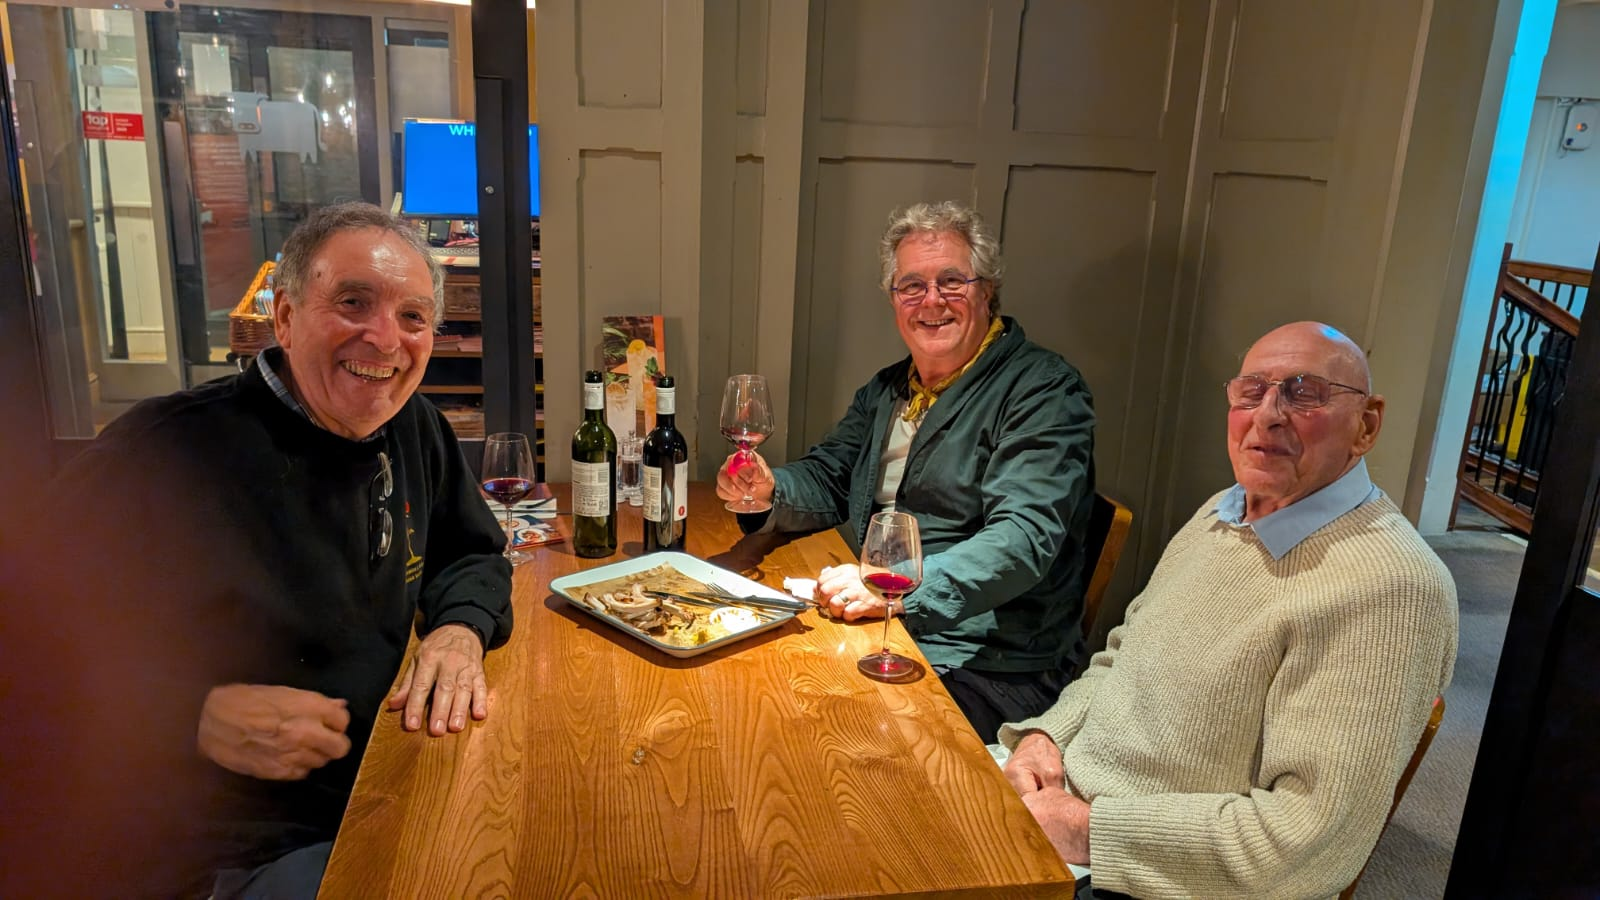
\includegraphics[angle=0,origin=c,width=1.0\textwidth]{2025_09/res/show_ea01.jpeg}
\end{minipage}\quad
\begin{minipage}[b]{.4\textwidth}
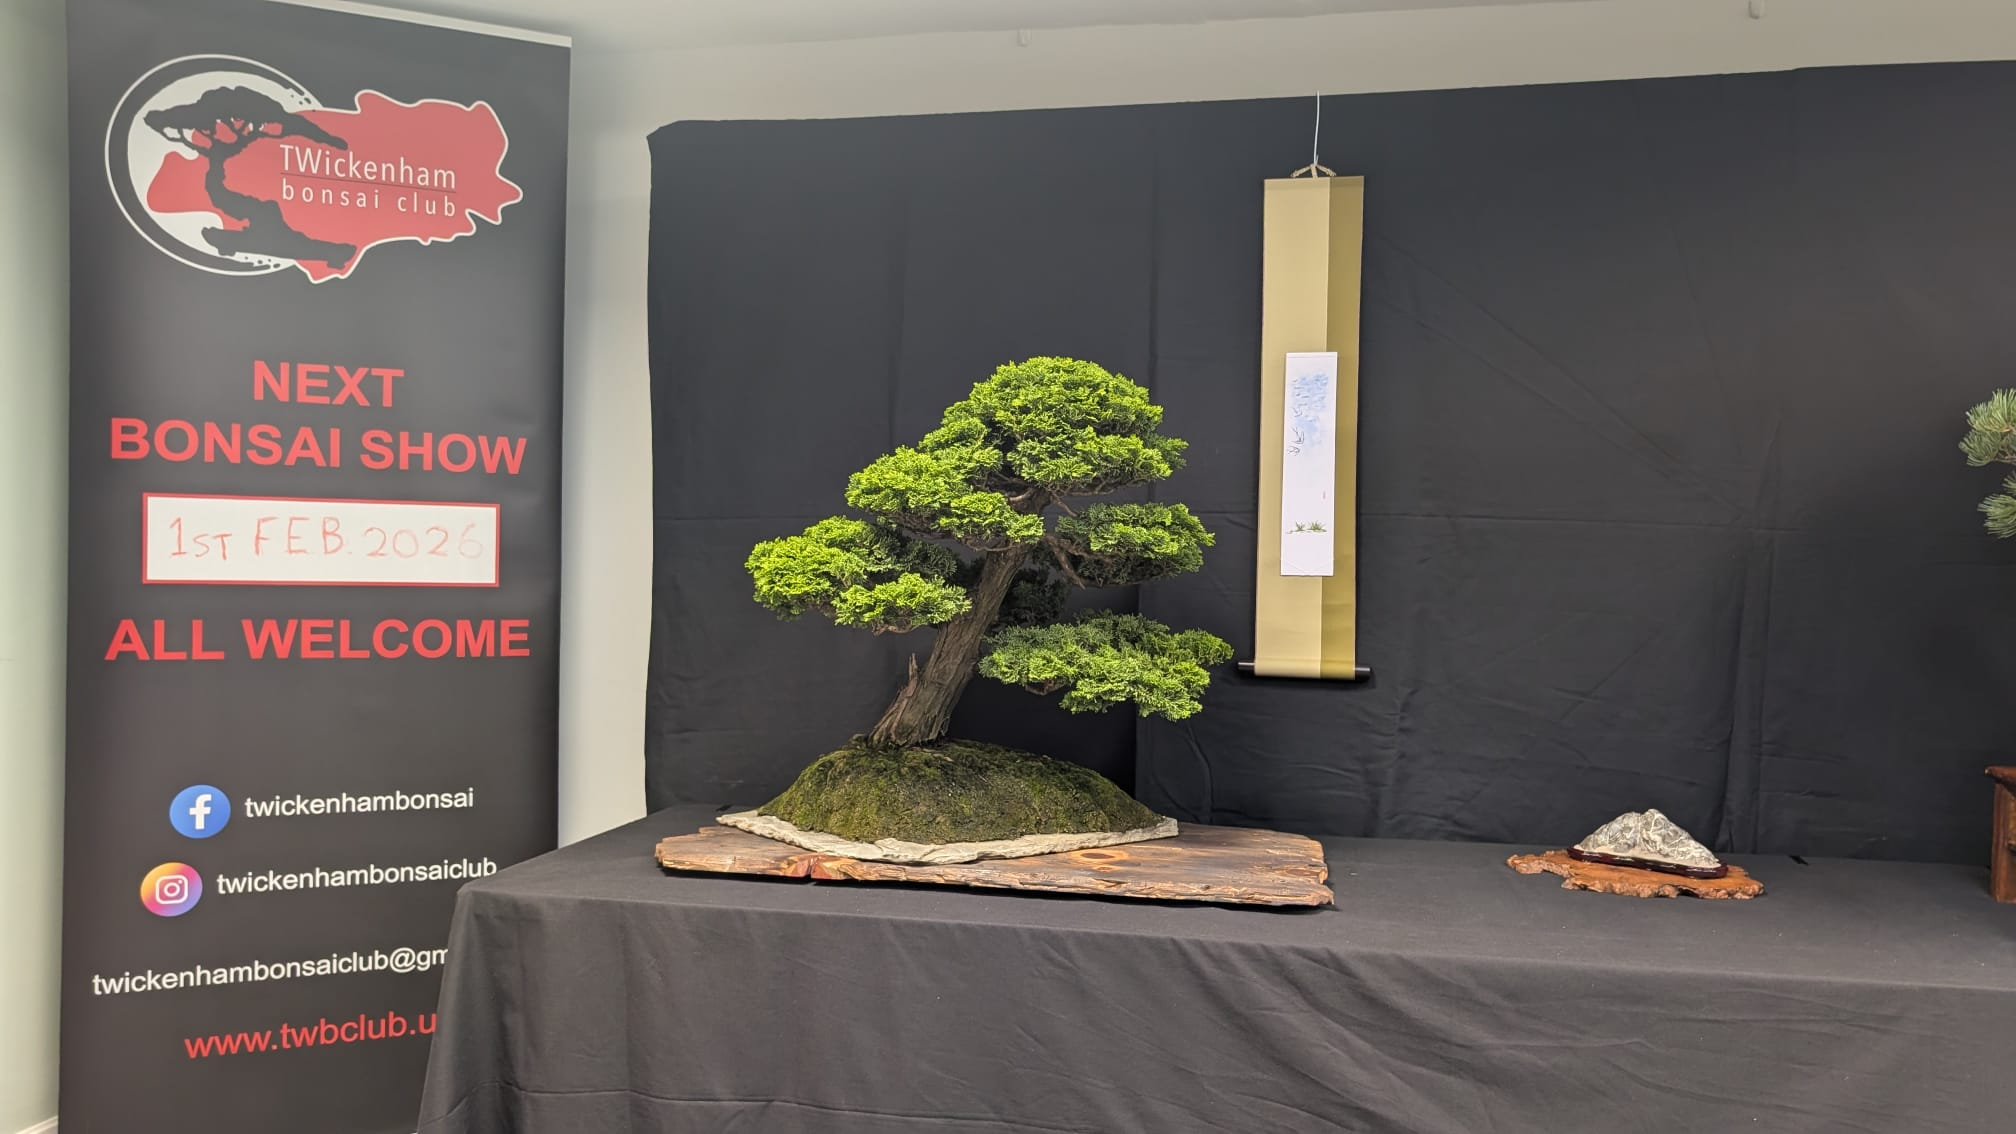
\includegraphics[angle=0,origin=c,width=1.0\textwidth]{2025_09/res/show_ea02.jpeg}
\end{minipage}
\medskip 

\begin{minipage}[b]{.4\textwidth}
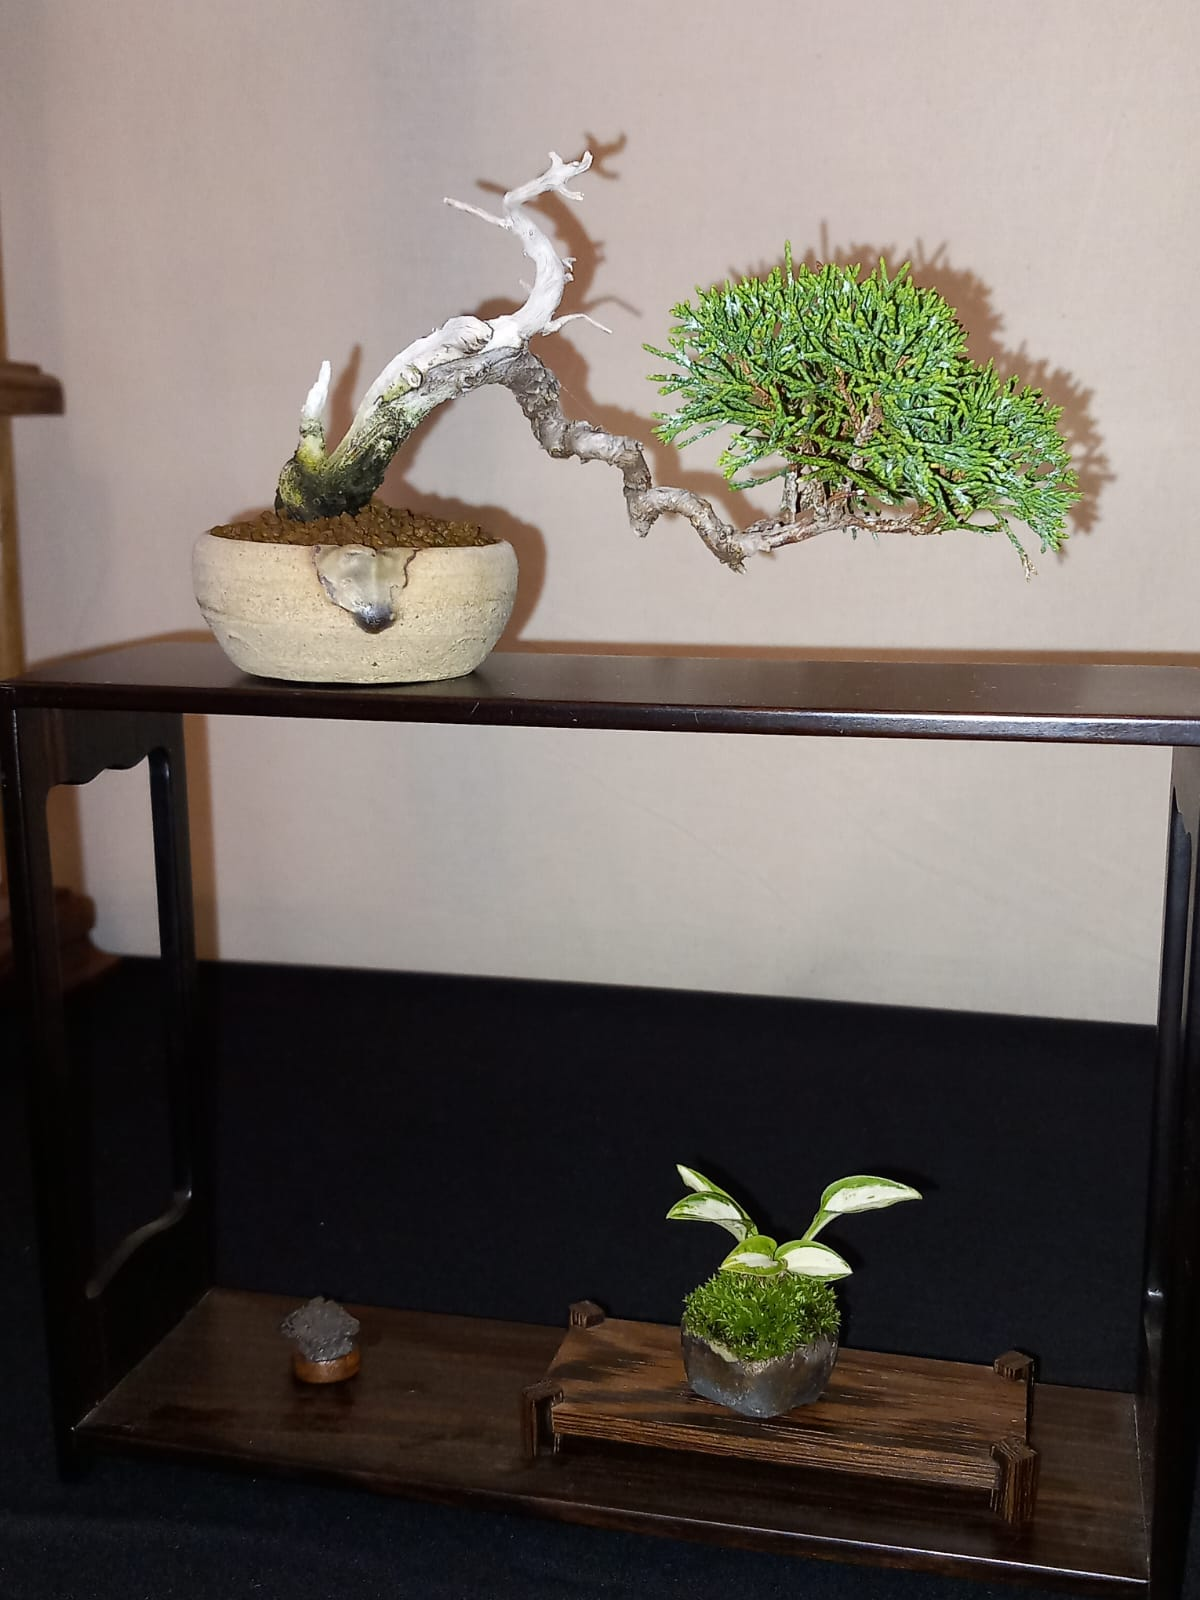
\includegraphics[angle=0,origin=c,width=1.0\textwidth]{2025_09/res/show_ea03.jpeg}
\end{minipage}\quad
\begin{minipage}[b]{.4\textwidth}
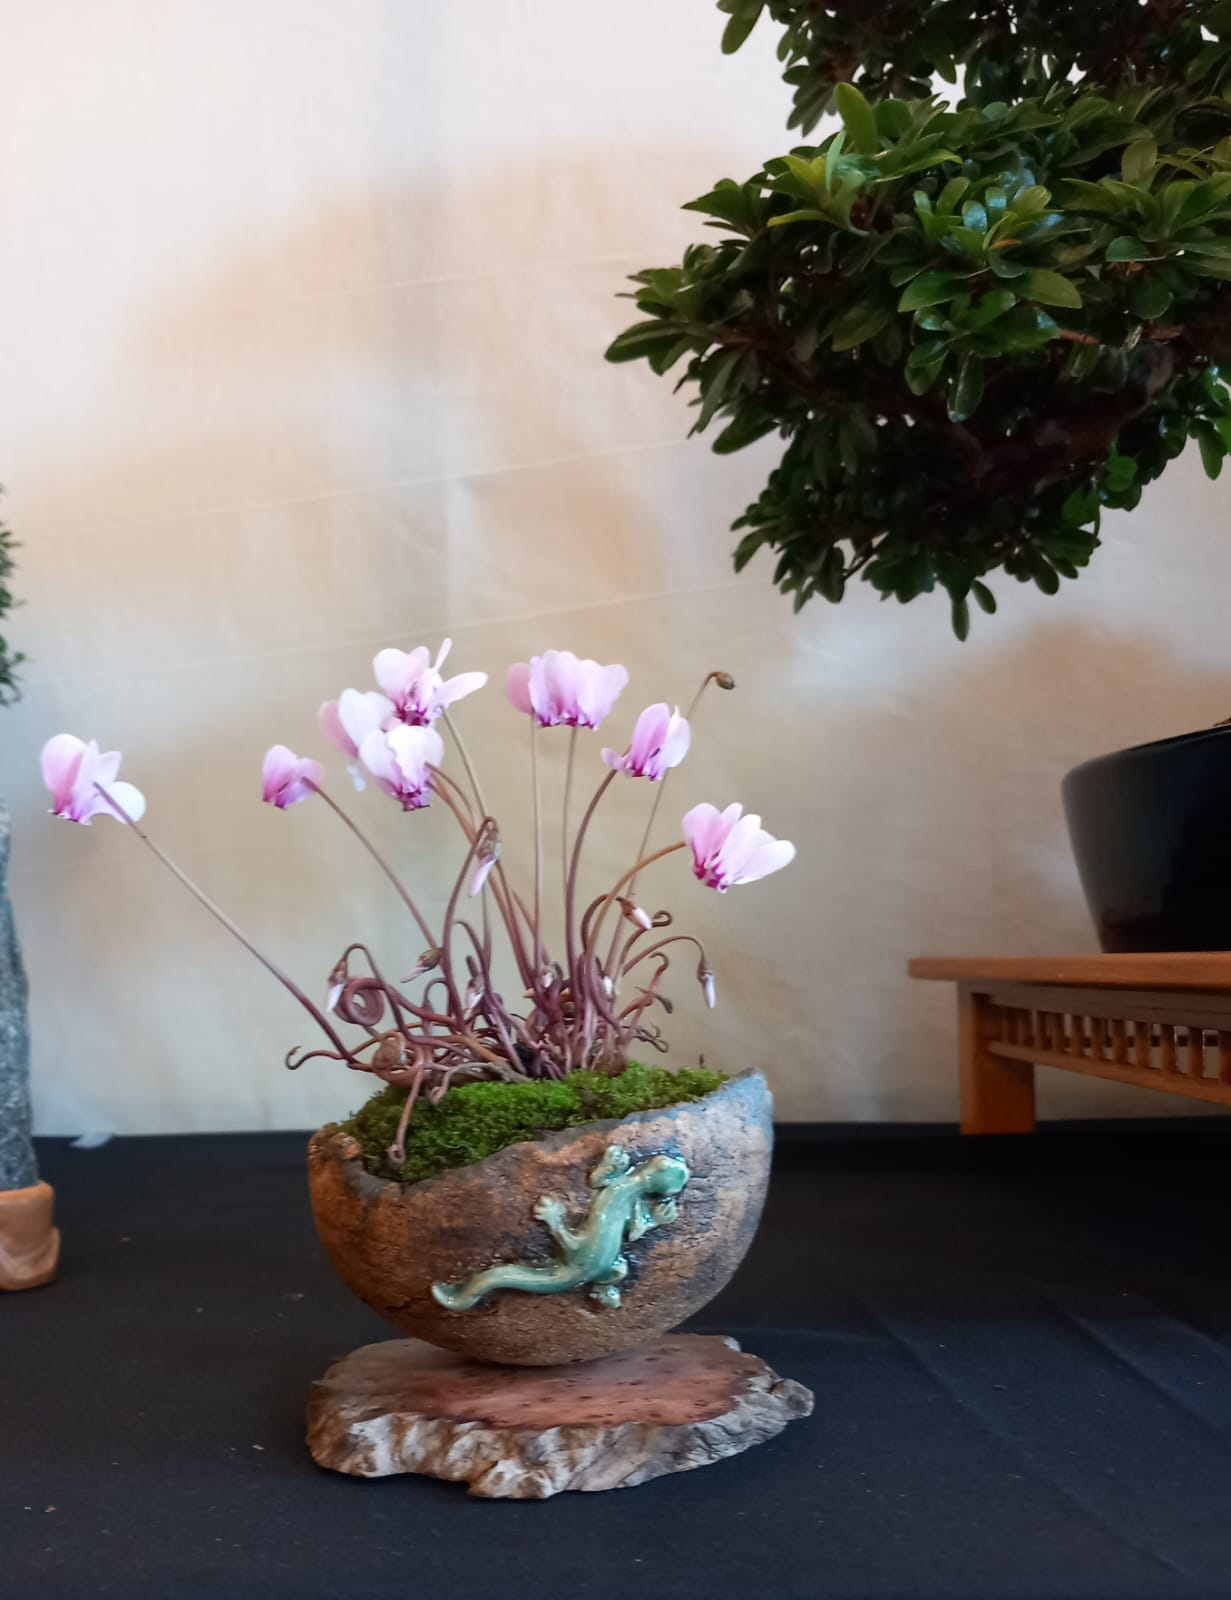
\includegraphics[angle=0,origin=c,width=1.0\textwidth]{2025_09/res/show_ea04.jpeg}
\end{minipage}
\medskip 

\begin{minipage}[b]{.4\textwidth}
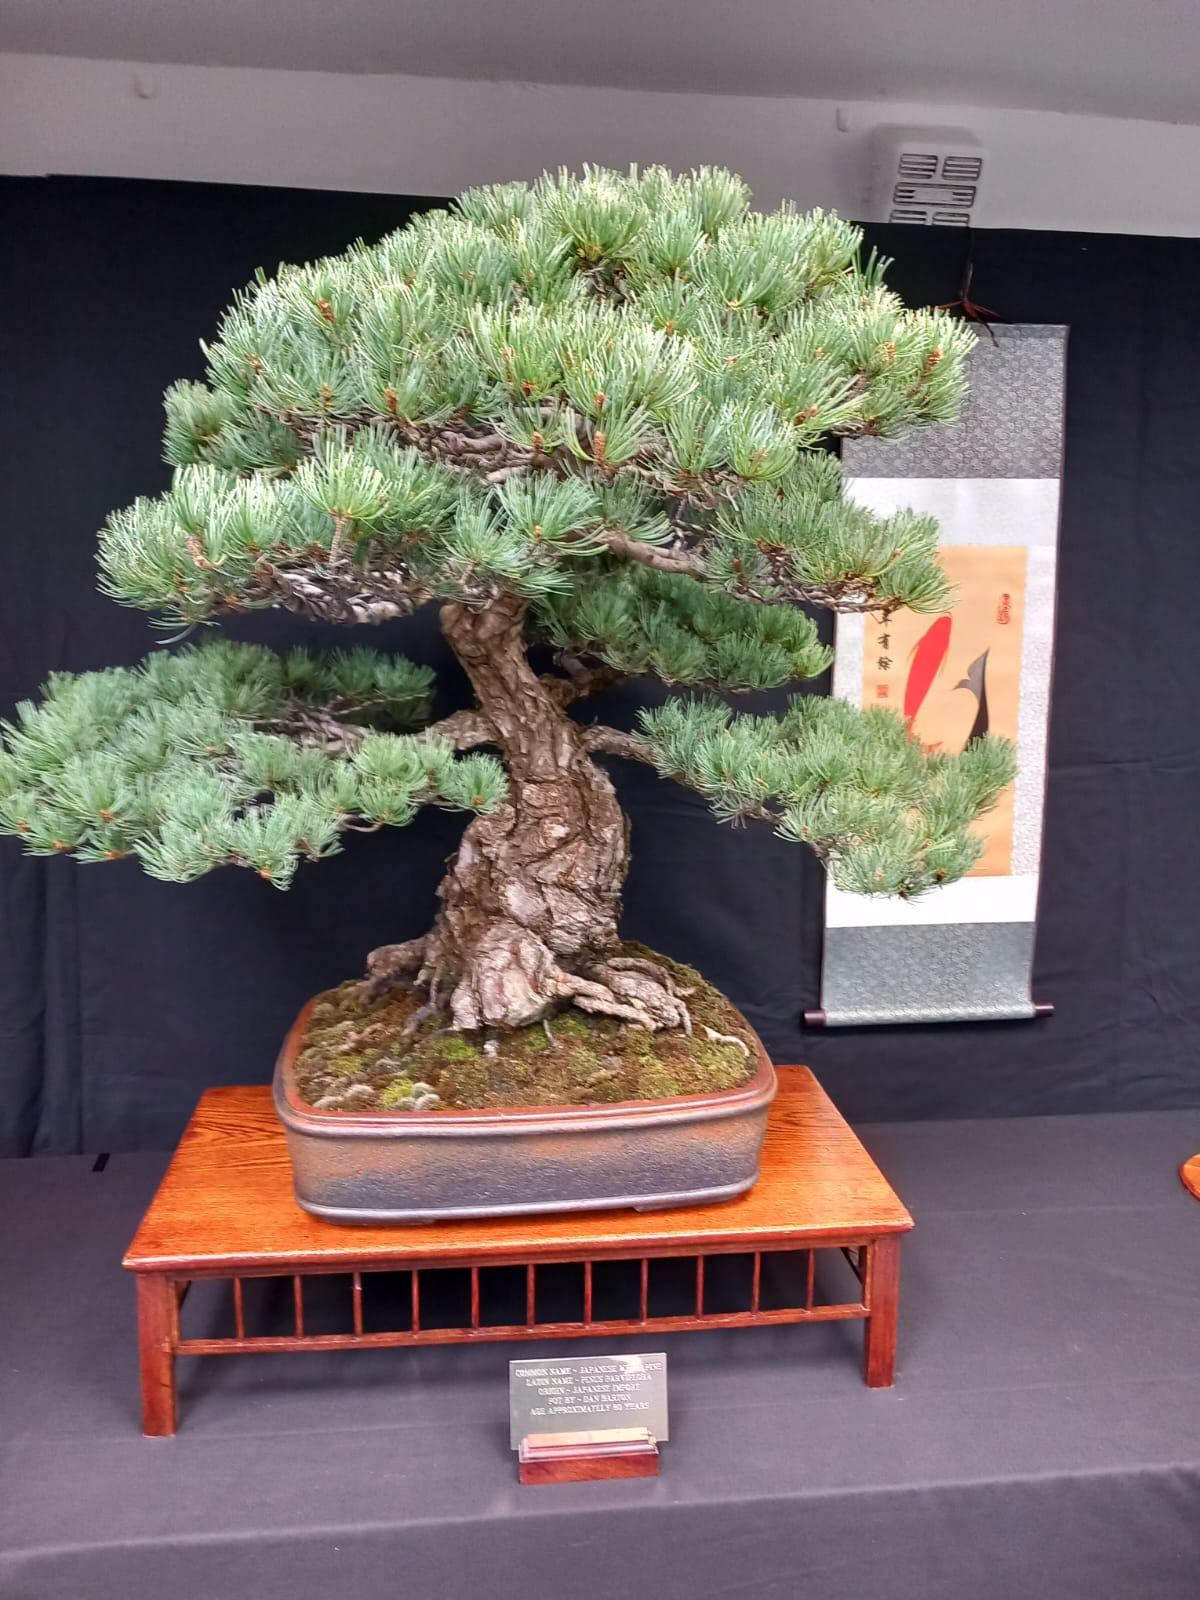
\includegraphics[angle=0,origin=c,width=1.0\textwidth]{2025_09/res/show_ea05.jpeg}
\end{minipage}\quad
\begin{minipage}[b]{.4\textwidth}
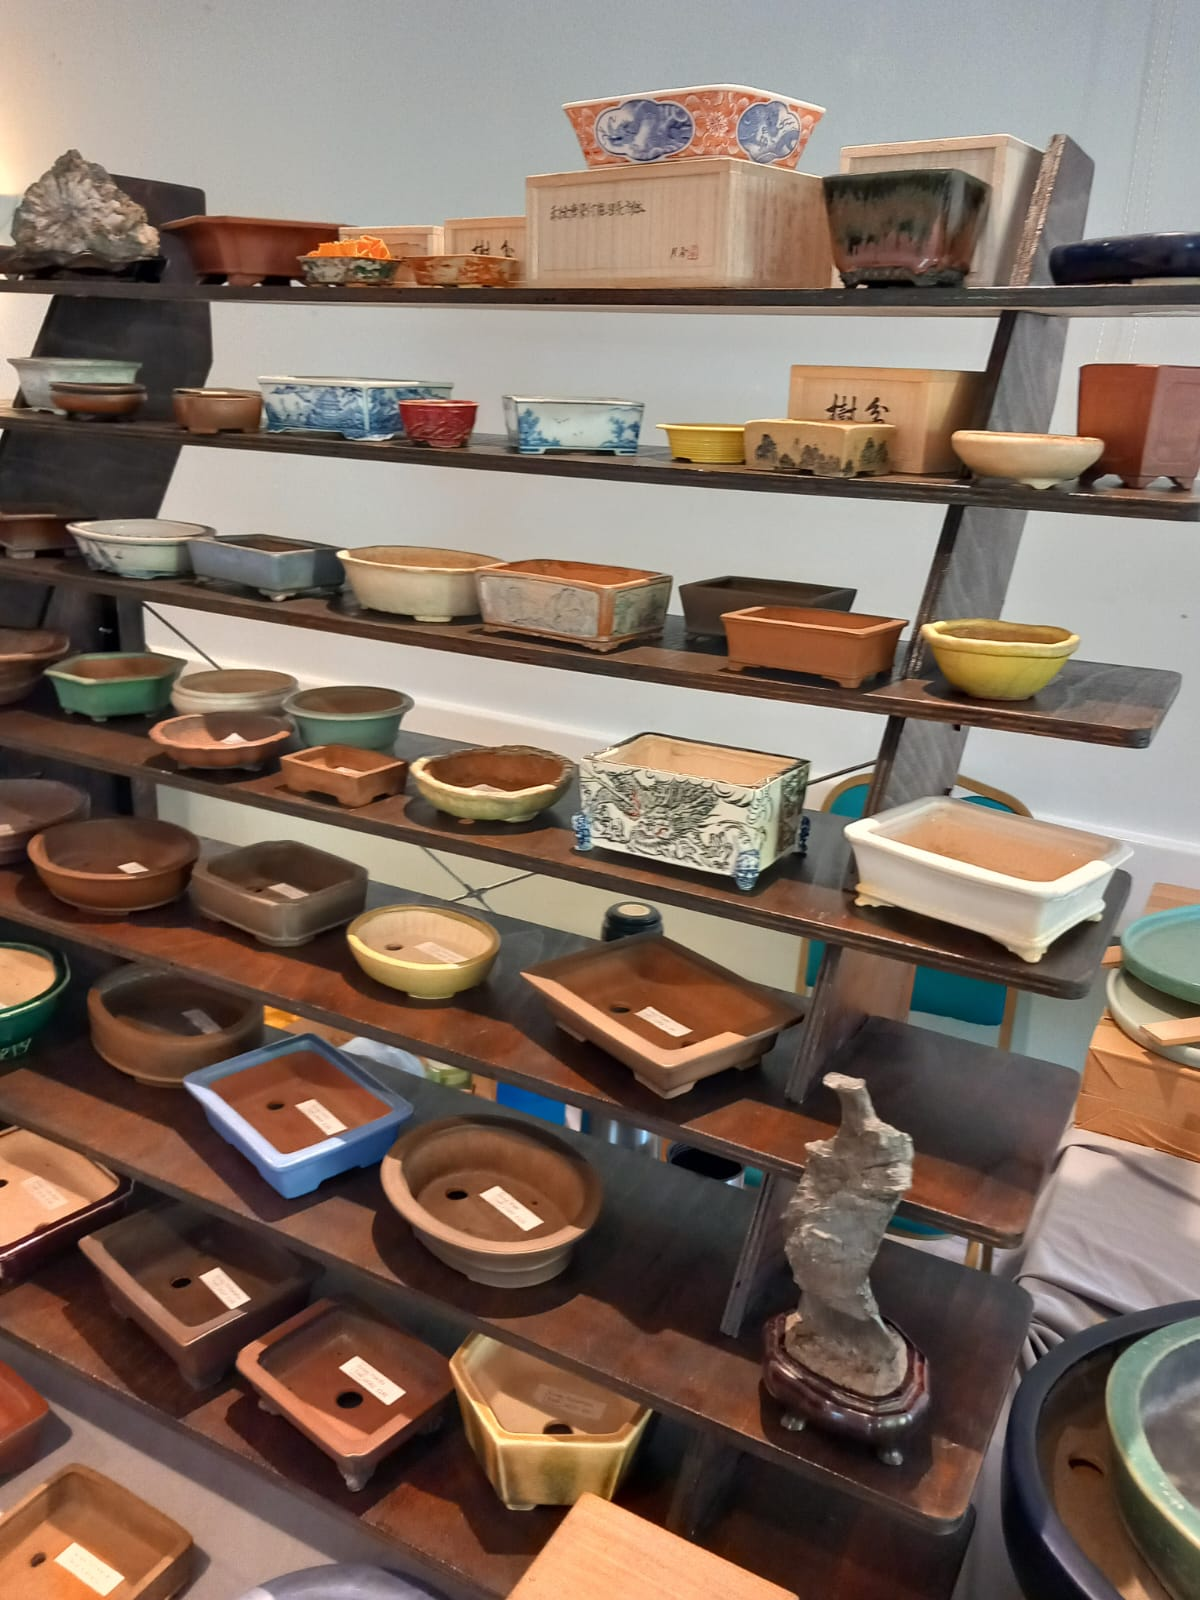
\includegraphics[angle=0,origin=c,width=1.0\textwidth]{2025_09/res/show_ea06.jpeg}
\end{minipage}
\medskip

\emph{A vibrant day in Kesgrave: trees, traders, tiny displays, and the thoughtful critique of a Hinoki cypress.}
\end{center}

\clearpage

\begin{center}
\begin{minipage}[b]{.4\textwidth}
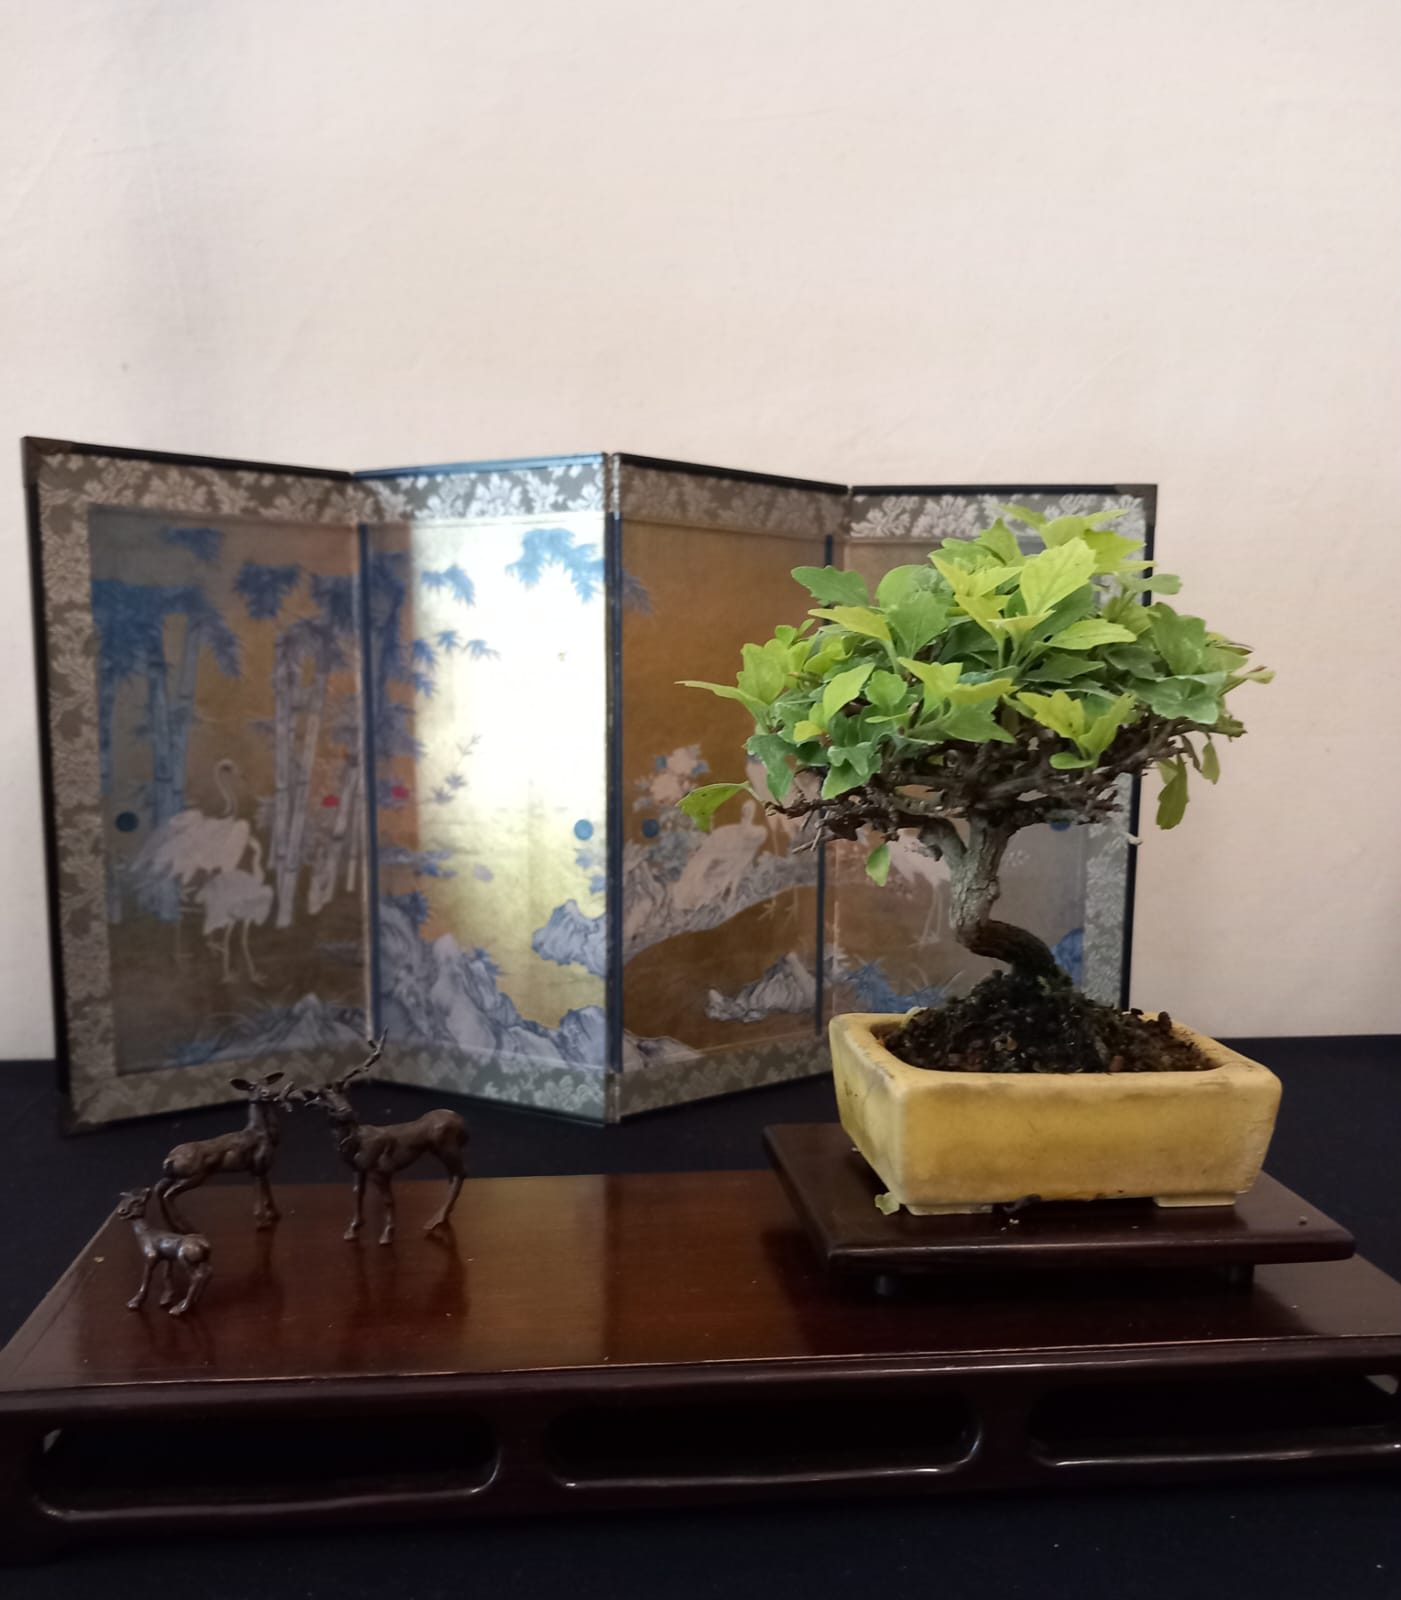
\includegraphics[angle=0,origin=c,width=1.0\textwidth]{2025_09/res/show_ea07.jpeg}
\end{minipage}\quad
\begin{minipage}[b]{.4\textwidth}
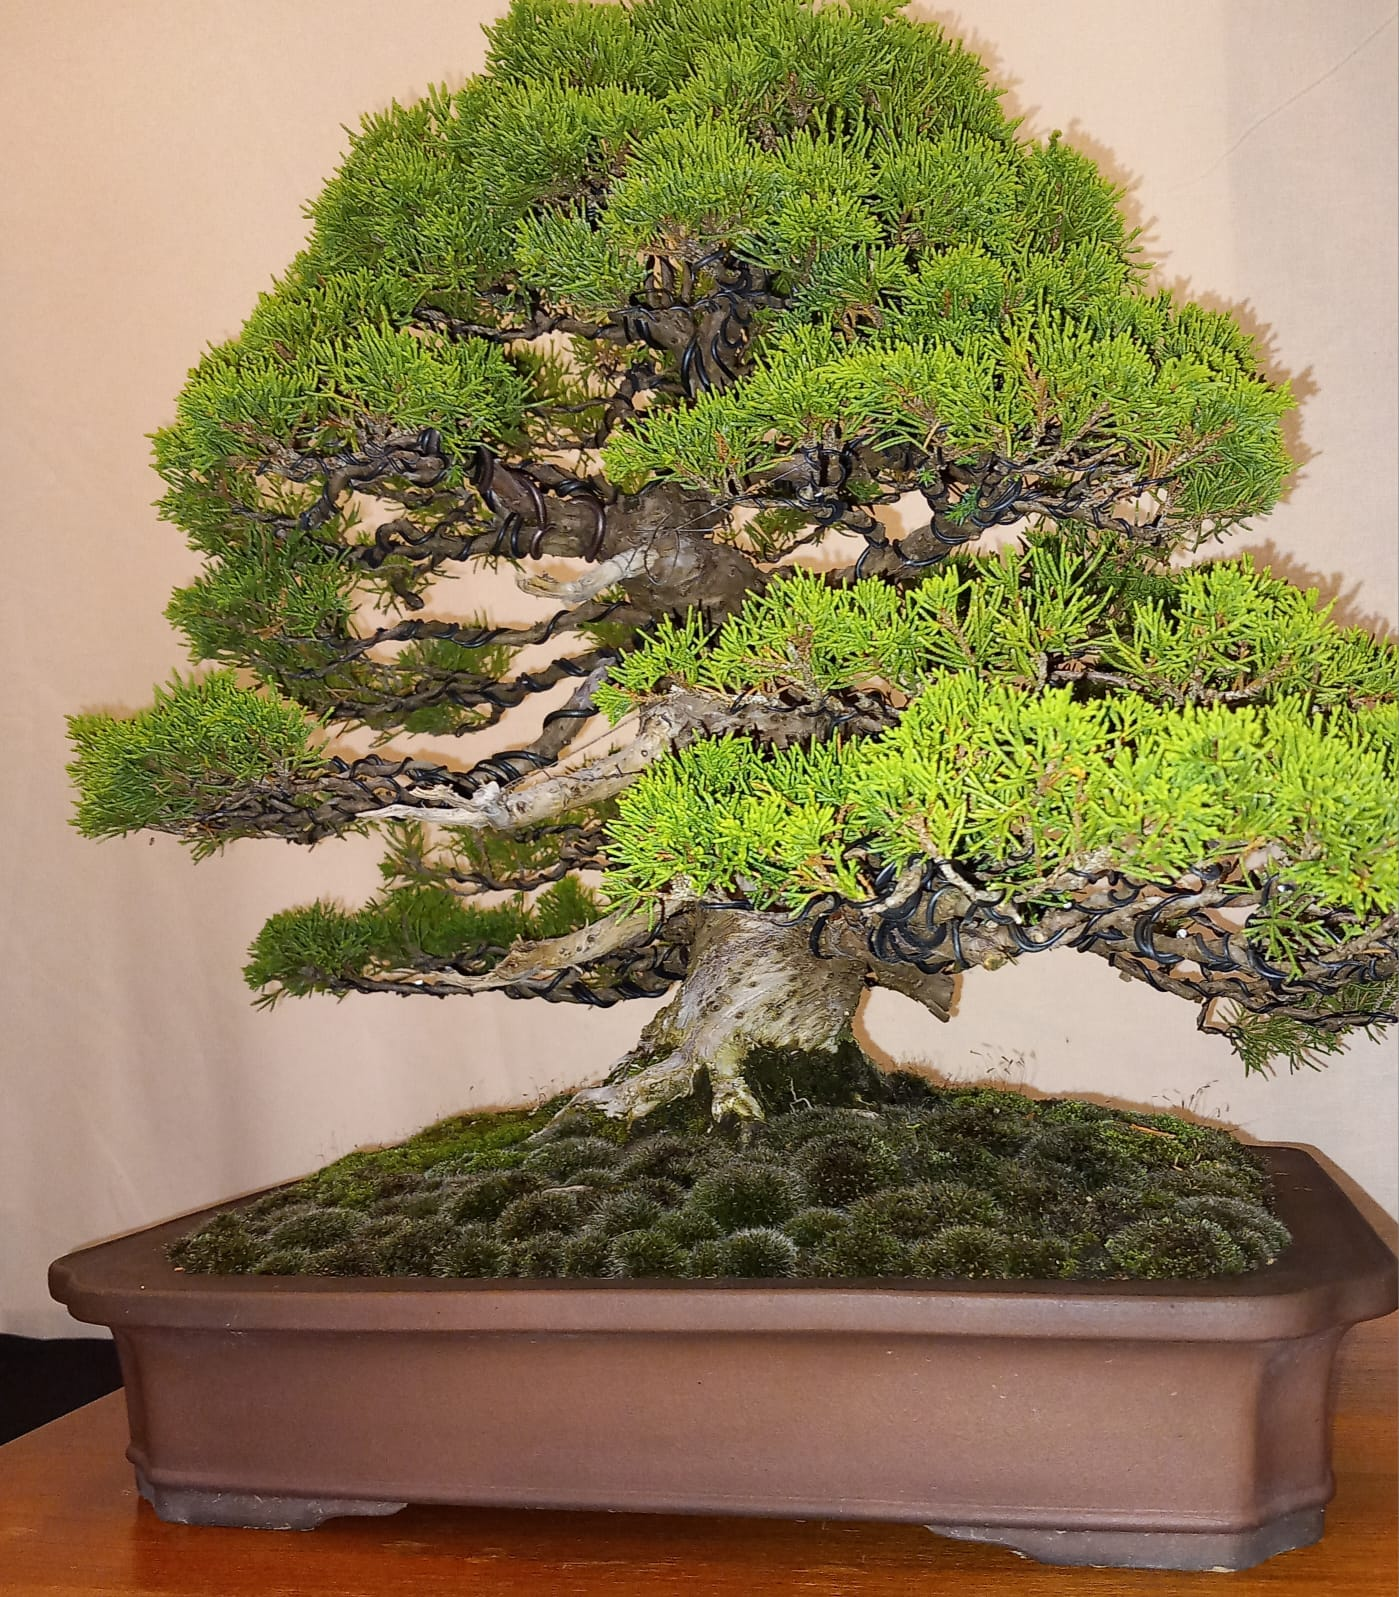
\includegraphics[angle=0,origin=c,width=1.0\textwidth]{2025_09/res/show_ea08.jpeg}
\end{minipage}
\medskip 

\begin{minipage}[b]{.4\textwidth}
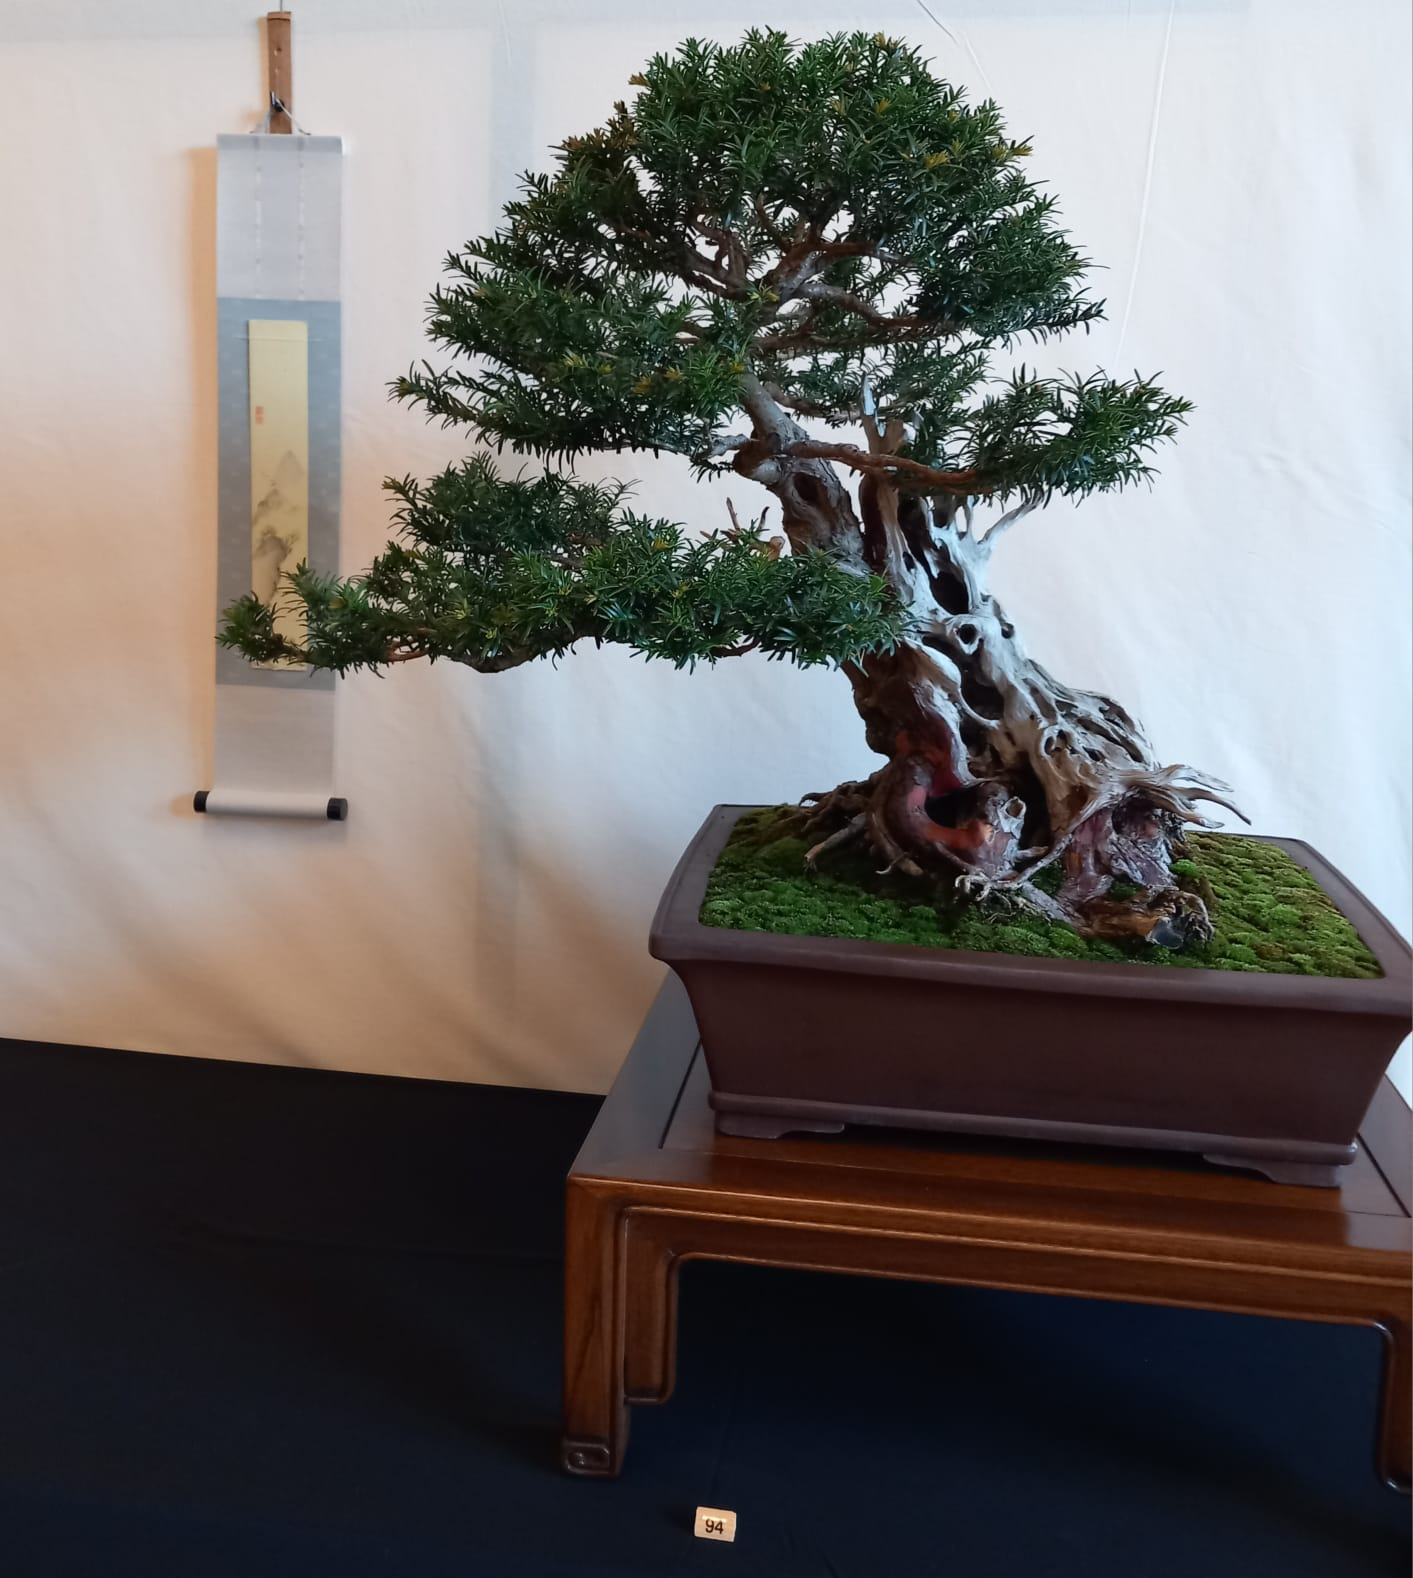
\includegraphics[angle=0,origin=c,width=1.0\textwidth]{2025_09/res/show_ea09.jpeg}
\end{minipage}\quad
\begin{minipage}[b]{.4\textwidth}
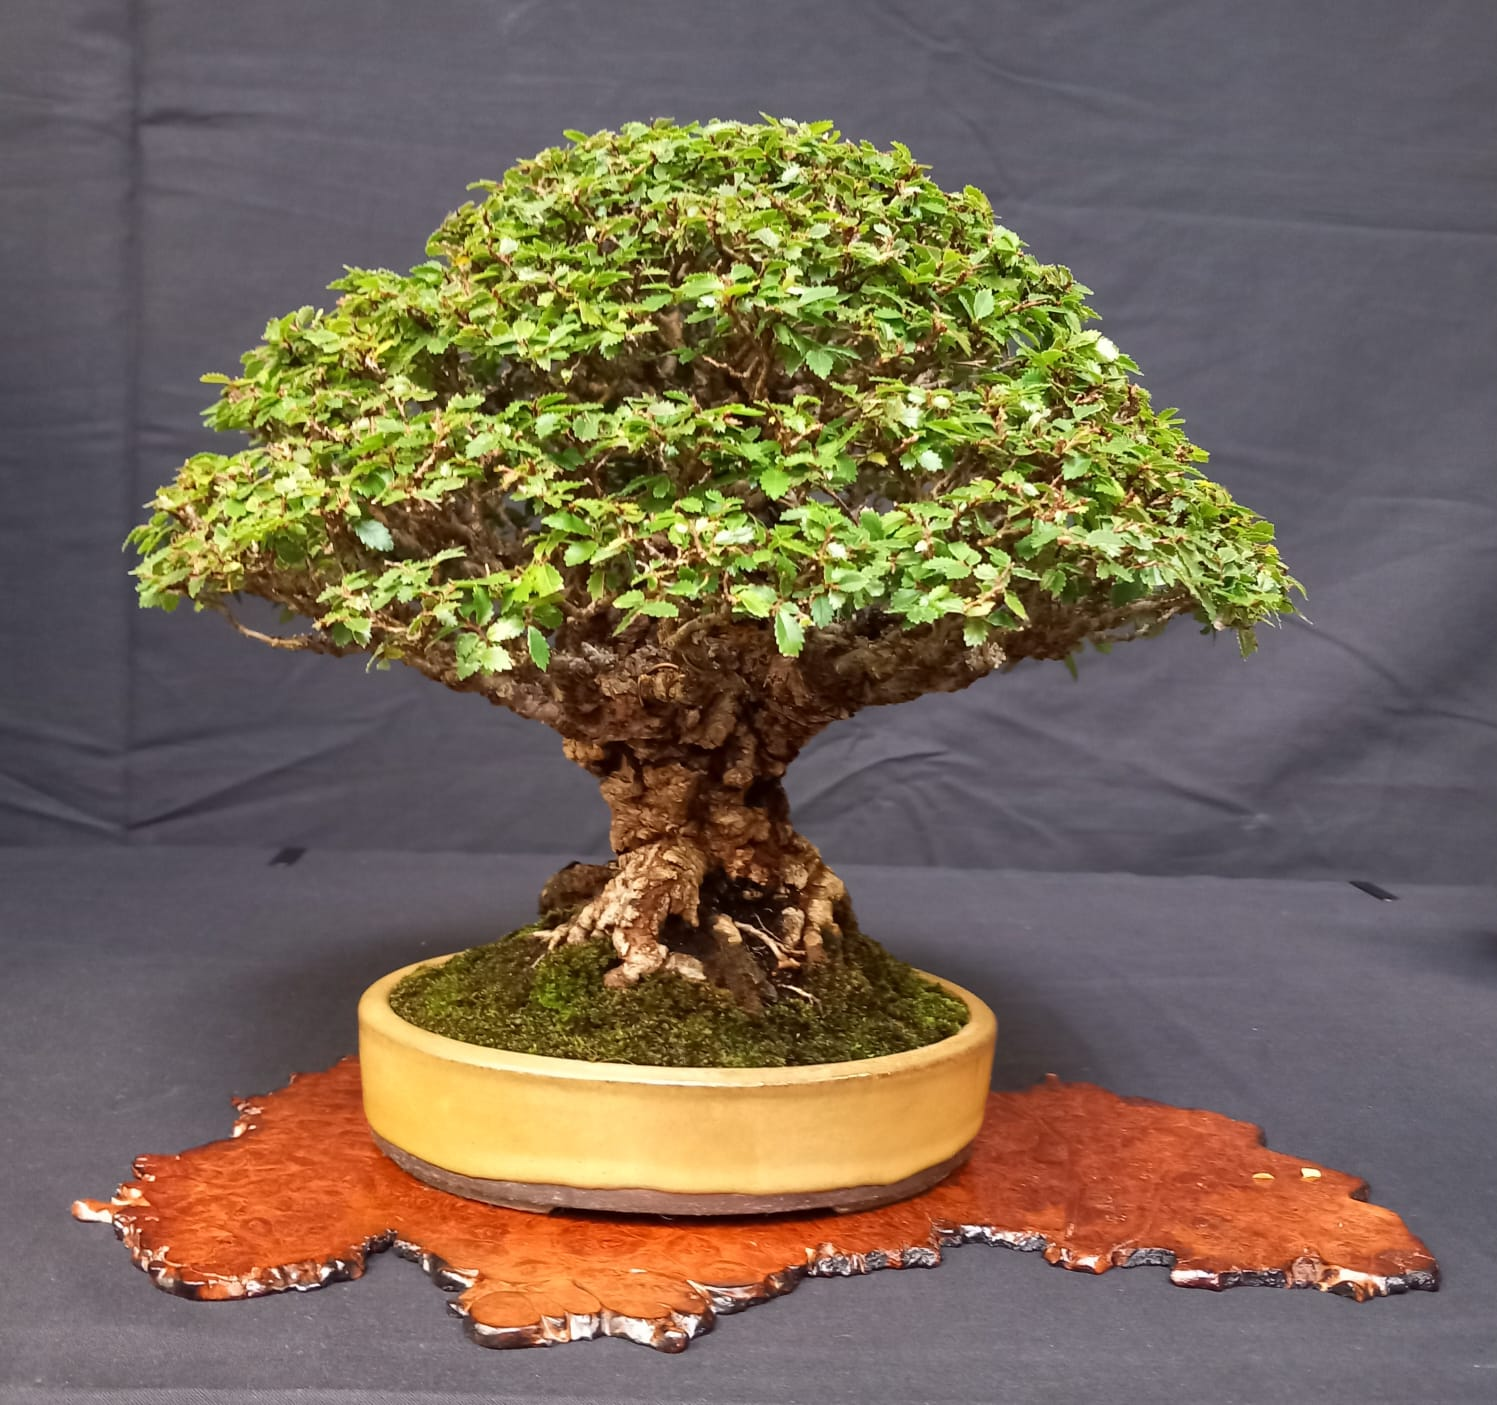
\includegraphics[angle=0,origin=c,width=1.0\textwidth]{2025_09/res/show_ea10.jpeg}
\end{minipage}
\medskip 

\begin{minipage}[b]{.4\textwidth}
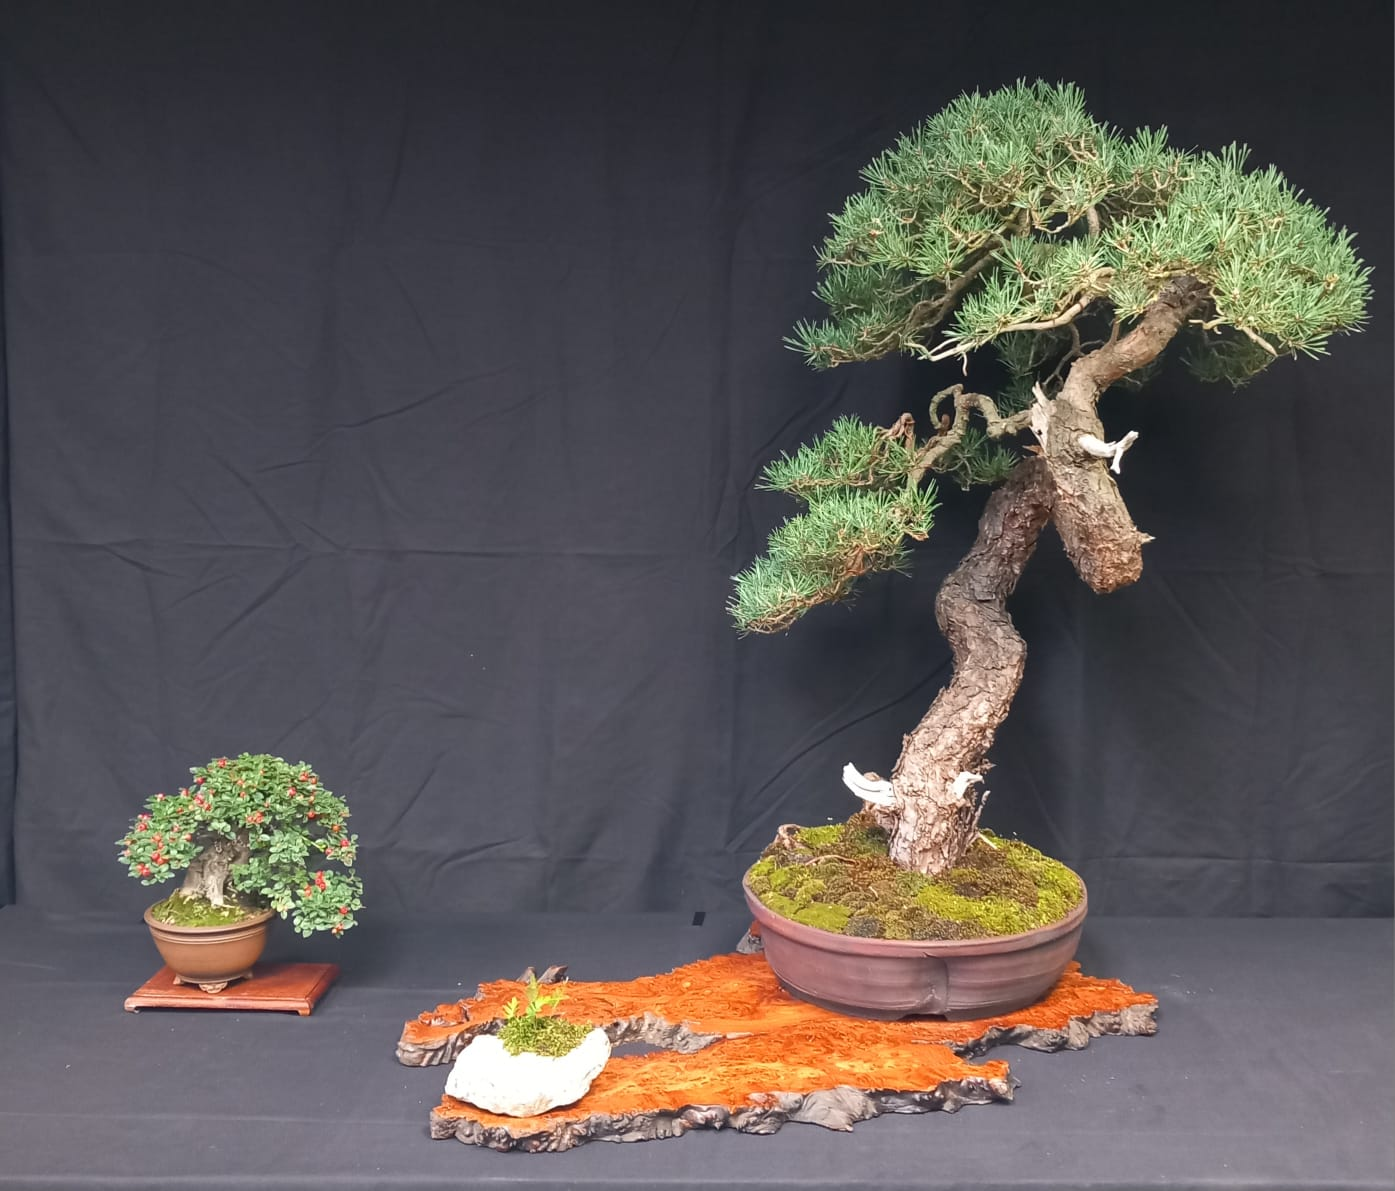
\includegraphics[angle=0,origin=c,width=1.0\textwidth]{2025_09/res/show_ea11.jpeg}
\end{minipage}\quad
\begin{minipage}[b]{.4\textwidth}
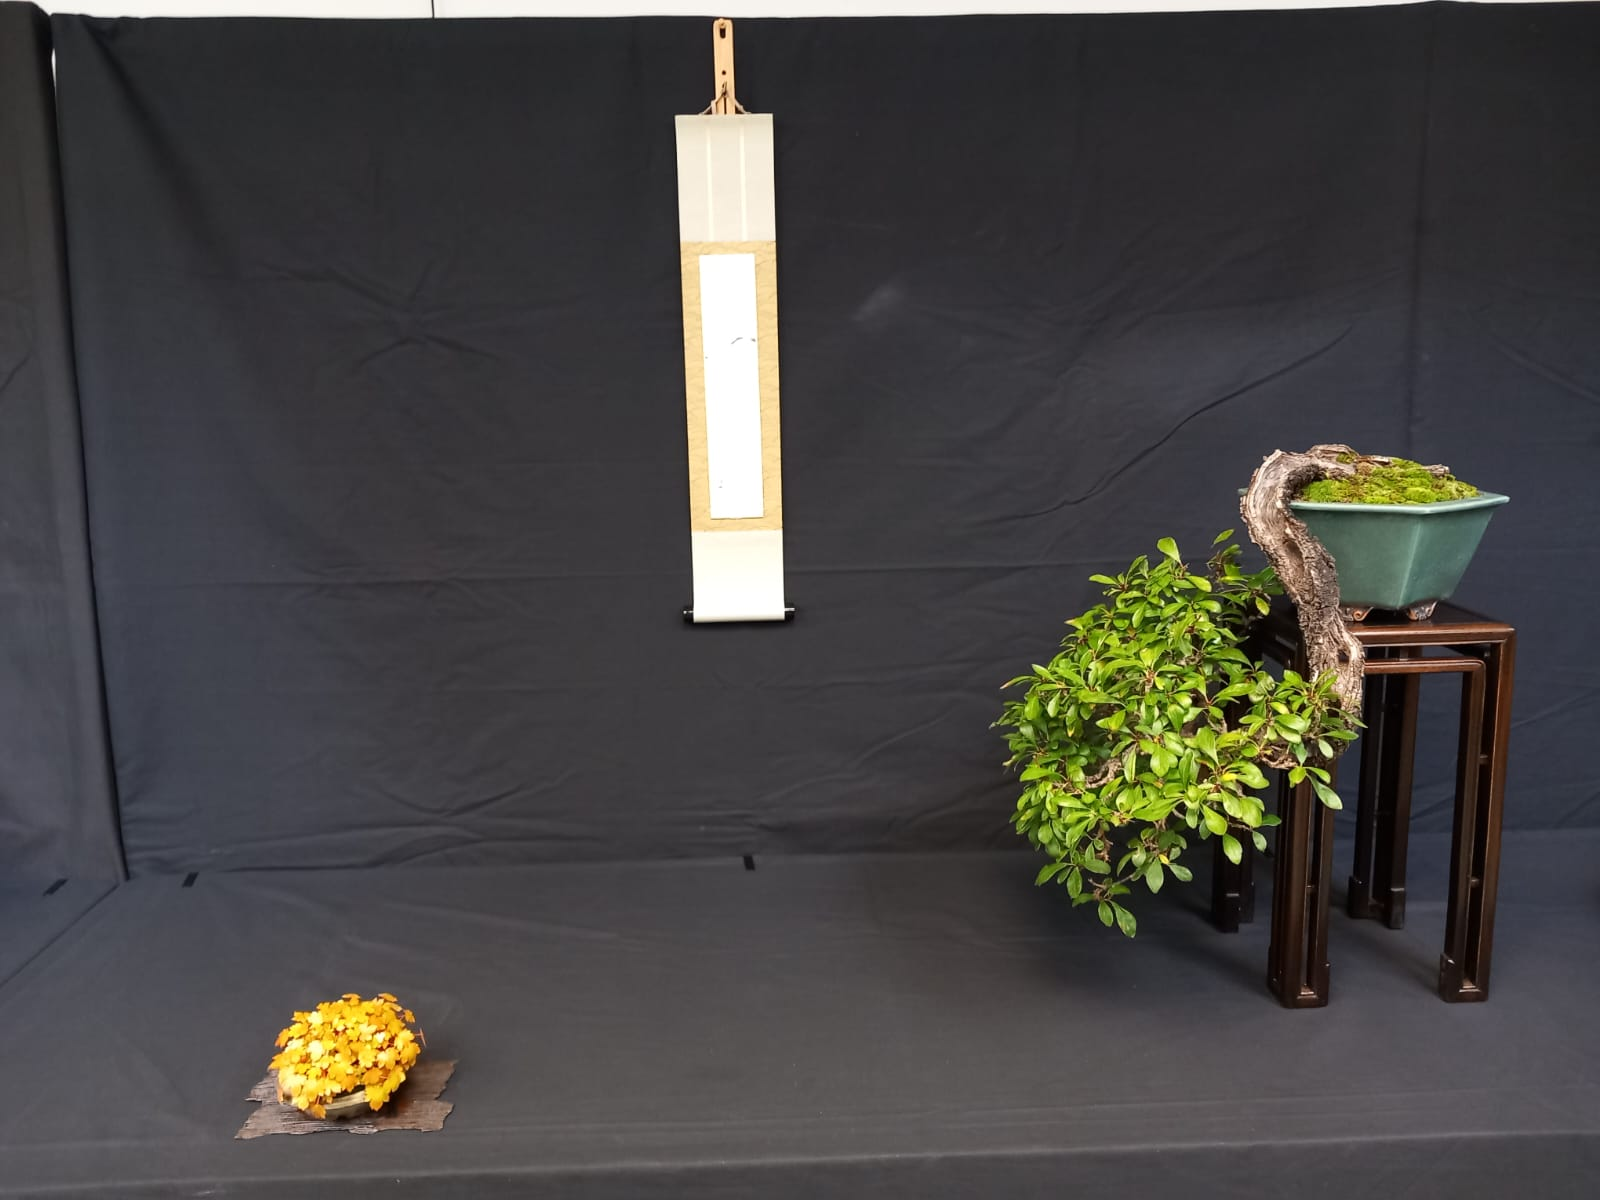
\includegraphics[angle=0,origin=c,width=1.0\textwidth]{2025_09/res/show_ea12.jpeg}
\end{minipage}
\medskip

\emph{A vibrant day in Kesgrave: trees, traders, tiny displays, and the thoughtful critique of a Hinoki cypress.}
\end{center}

\clearpage
\begin{multicols}{2}{
